\documentclass{article}
\usepackage[utf8]{inputenc}
\usepackage[margin=1in]{geometry}

\title{452 - Homework 4}
\author{Victor Zhang}
\date{February 19, 2021}

\usepackage[utf8]{inputenc}
\usepackage{amsmath}
\usepackage{amsfonts}
\usepackage{natbib}
\usepackage{graphicx}
% \usepackage{changepage}
\usepackage{amssymb}
\usepackage{xfrac}
% \usepackage{bm}
% \usepackage{empheq}
\usepackage{dirtytalk}

\usepackage{tikz}
\usetikzlibrary{arrows,automata,shapes}

\newcommand{\contra}{\raisebox{\depth}{\#}}

\newenvironment{myindentpar}[1]
  {\begin{list}{}
          {\setlength{\leftmargin}{#1}}
          \item[]
  }
  {\end{list}}

\pagestyle{empty}

\begin{document}

\maketitle
% \begin{center}
% {\huge Econ 482 \hspace{0.5cm} HW 3}\
% {\Large \textbf{Victor Zhang}}\
% {\Large February 18, 2020}
% \end{center}

\section*{2.4.e}
Let $G = (\{S\},\Sigma,R,S)$ where the ruleset $R$ is given
\begin{equation*}
\begin{cases}
S \to 1S1 \;\vert\; 0S0\\
S \to 1 \;\vert\; 0 \;\vert\; \epsilon
\end{cases}
\end{equation*}
To show $G$ generates all the palindromes, it suffices to note the first and last characters of a palindrome must be the same, and the inner characters form a palindrome. The first rule represents this recursion and the second represents the base cases $\Box$

\section*{2.5.e}
The following is a pushdown automaton that accepts palindromes:\\
The start state branches into two submachines: one that deals with even-length palindromes and one that deals with odd-length palindromes. Within the even submachine, push incoming symbols onto the stack until we get to the middle of the string, then compare incoming symbols with the stack top and pop if they match. Similarly with the odd submachine, except between the pushing and popping, read in one \say{middle} symbol.

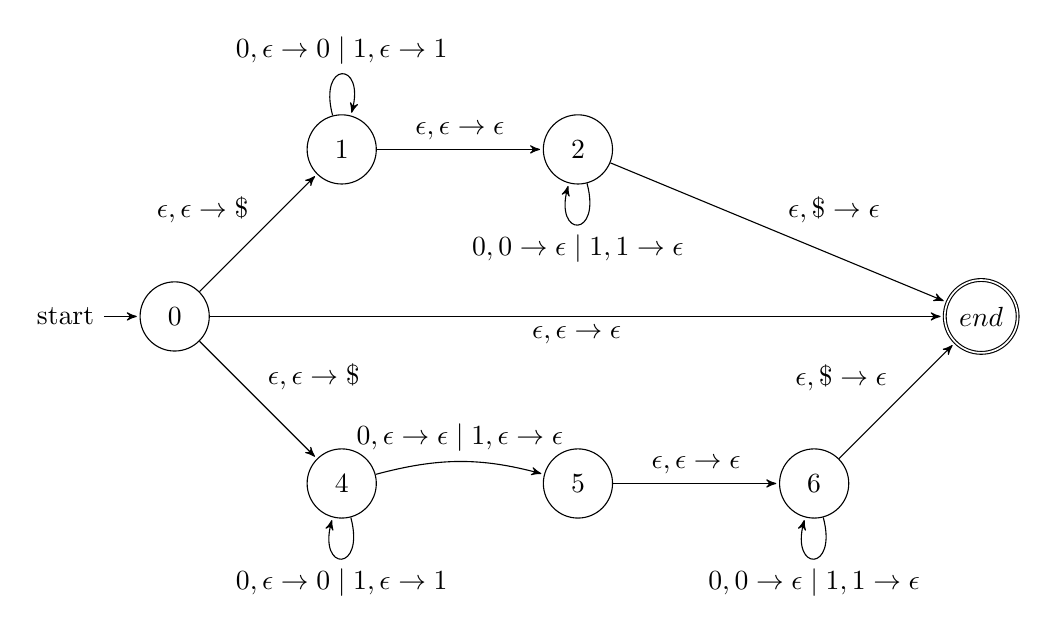
\begin{tikzpicture}[->,>=stealth',shorten >=1pt,auto,node distance=3cm,
        scale = 1,transform shape]

  \node[state,initial] (0) {$0$};
  \node[state] (1) [above right of=0] {$1$};
  \node[state] (2) [right of=1] {$2$};
  \node[state] (4) [below right of=0] {$4$};
  \node[state] (5) [right of=4] {$5$};
  \node[state] (6) [right of=5] {$6$};
  \node[state,accepting] (end) [above right of=6] {$end$};

  \path (0) edge              node {$\epsilon,\epsilon\to\$$} (1)
        (0) edge              node {$\epsilon,\epsilon\to\$$} (4)
        (1) edge [loop above] node {$0,\epsilon\to 0\;|\;1,\epsilon \to 1$} (1)
        (4) edge [loop below] node {$0,\epsilon\to 0\;|\;1,\epsilon \to 1$} (4)
        (4) edge [bend left=15] node {$0,\epsilon\to \epsilon\;|\;1,\epsilon \to \epsilon$} (5)
        (1) edge              node {$\epsilon,\epsilon\to \epsilon$} (2)
        (5) edge              node {$\epsilon,\epsilon\to \epsilon$} (6)
        (2) edge [loop below] node {$0,0\to\epsilon\;|\;1,1\to\epsilon$} (2)
        (6) edge [loop below] node {$0,0\to\epsilon\;|\;1,1\to\epsilon$} (6)
        (2) edge              node {$\epsilon,\$\to\epsilon$} (end)
        (6) edge              node {$\epsilon,\$\to\epsilon$} (end)
        (0) edge              node [below] {$\epsilon,\epsilon\to\epsilon$} (end);

\end{tikzpicture}

\section*{2.9}
Let $G = (\{S,A,B,C,E,F,G\},\{a,b,c\},R,S)$ where the ruleset $R$ is given
\begin{equation*}
\begin{cases}
S \to A \;|\; E\\
A \to BC\\
B \to aBb \;|\; \epsilon\\
C \to cC \;|\; \epsilon\\
E \to FG\\
F \to aF \;|\; \epsilon\\
G \to bGc \;|\; \epsilon
\end{cases}
\end{equation*}
This grammar clearly derives $A$, including when any or all of $i,j,k$ are 0.
This grammar is ambiguous, necessarily so, since the string $\epsilon$ may be derived $S \to A \to BC \to \epsilon\epsilon$ or $S \to E \to FG \to \epsilon\epsilon$ $\Box$

\section*{2.10}
The starting state branches into two submachines, one that handles $i=j$ and another that handles $j=k$. Within the first submachine, embed a PDA $AB$ that accepts strings of the form $a^nb^n$, perhaps according to example 2.14 in the text. The accepting state of this PDA is piped into an accepting state that accepts some or no input symbols $c$. The second submachine consists of a state that accepts some or no input symbols $a$ and transitions (on the empty string) to a PDA $BC$ that accepts strings of the form $b^nc^n$. An informal state diagram for this machine is included below

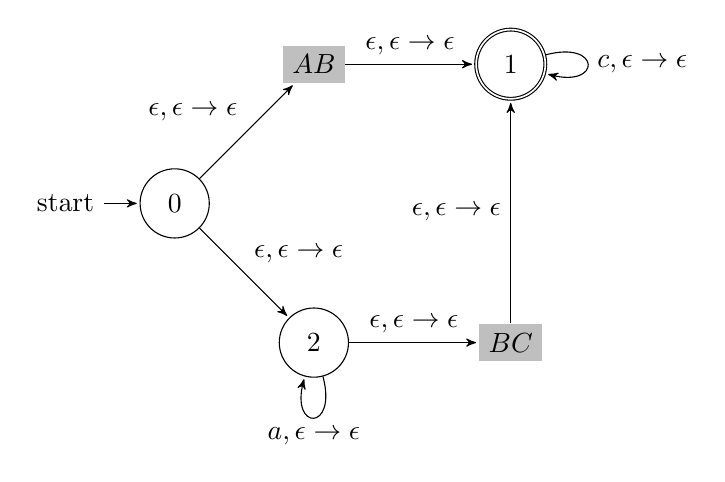
\begin{tikzpicture}[->,>=stealth',shorten >=1pt,auto,node distance=2.5cm,
        scale = 1,transform shape]

  \node[state,initial] (0) {$0$};
  \node[rectangle,fill=lightgray] (AB) [above right of=0] {$AB$};
  \node[state,accepting] (1) [right of=AB] {$1$};
  \node[state] (2) [below right of=0] {$2$};
  \node[rectangle,fill=lightgray] (BC) [right of=2] {$BC$};

  \path (0) edge              node {$\epsilon,\epsilon\to\epsilon$} (AB)
        (0) edge              node {$\epsilon,\epsilon\to\epsilon$} (2)
        (AB) edge              node {$\epsilon,\epsilon\to\epsilon$} (1)
        (1) edge [loop right] node {$c,\epsilon\to\epsilon$} (1)
        (2) edge              node {$\epsilon,\epsilon\to\epsilon$} (BC)
        (2) edge [loop below] node {$a,\epsilon\to\epsilon$} (2)
        (BC) edge              node {$\epsilon,\epsilon\to\epsilon$} (1);

\end{tikzpicture}

\section*{2.14}
We assume the starting string is $A$. Otherwise we may remove the first rule to get a CFG in Chomsky normal form.
\begin{equation*}
\begin{cases}
A \to BAB \;|\; B \;|\; \epsilon\\
B \to 00 \;|\; \epsilon
\end{cases}
\to
\begin{cases}
A \to BAB \;|\; B \;|\; \epsilon\\
B \to DD\\
D \to 0\\
\end{cases}
\to
\begin{cases}
A \to EB \;|\; DD \;|\; \epsilon\\
B \to DD\\
D \to 0\\
E \to BA\\
\end{cases}
\to
\begin{cases}
S \to A \;|\; \epsilon\\
A \to EB \;|\; DD\\
B \to DD\\
D \to 0\\
E \to BA\\
\end{cases}
\end{equation*}
Where in the new CFG, $S$ is the starting symbol $\Box$

\section*{2.35}
Chomsky normal form ensures rules with predicate not the starting symbol never derive the empty string. Thus, if there is a \say{loop} in symbols, we may pump this loop and generate infinitely many strings of different lengths. More formally, if we may find some derivation $A \overset{*}{\to} V^+AV^*$ or $A \overset{*}{\to} V^*AV^+$ for symbol $A \in V$, $L(G)$ is infinite. If string $s$ is derived in $2^b$ steps, at most half of these steps can be steps between variables and terminals. Suppose $L(G)$ is finite. Then the derivation of $s$ contains at least $2^{b-1}$ rules of the form $A \to BC$ that do not generate a loop in symbols. This is impossible. Consider the (binary) parse tree of $s$. At each level $i$, we must introduce at least one new variable not seen in levels $j < i$, otherwise we will develop a loop. If we only have $b$ states, this restricts the parse tree to containl at most $b$ levels with variables (including the first level, with the starting symbol). Then there are at most $2^{b-1}-1$ distinct rules $A \to BC$, one less than we require $\Box$

\section*{CYK Algorithm}
The first string generates \verb|dp| table

\begin{tabular}{|*5{c|}}
\cline{1-1}
$S$&\multicolumn{4}{c}{}\\
\cline{1-2}
&$B$&\multicolumn{3}{c}{}\\
\cline{1-3}
$S$&$S$&$S$&\multicolumn{2}{c}{}\\
\cline{1-4}
&$B$&$B$&$B$&\multicolumn{1}{c}{}\\
\cline{1-5}
$C$&$S,A$&$S,A$&$S,A$&$C$\\
\hline
c&a&a&a&c\\
\end{tabular}

\noindent
so is generated by the grammar.\\\\
The second string generates \verb|dp| table

\begin{tabular}{|*5{c|}}
\cline{1-1}
&\multicolumn{4}{c}{}\\
\cline{1-2}
&$B$&\multicolumn{3}{c}{}\\
\cline{1-3}
&$S$&$S$&\multicolumn{2}{c}{}\\
\cline{1-4}
&$B$&$B$&$B$&\multicolumn{1}{c}{}\\
\cline{1-5}
$S$&$S,A$&$S,A$&$S,A$&$C$\\
\hline
c&a&a&a&c\\
\end{tabular}

\noindent
so is not generated by the grammar $\Box$

\end{document}

% List of tex snippets:
%   - tex-header (this)
%   - R      --> \mathbb{R}
%   - Z      --> \mathbb{Z}
%   - B      --> \mathcal{B}
%   - E      --> \mathcal{E}
%   - M      --> \mathcal{M}
%   - m      --> \mathfrak{m}({#1})
%   - normlp --> \norm{{#1}}_{L^{{#2}}}
